\chapter{Thực nghiệm và kết quả}
\label{chap:exp}

Chương này trình bày kết quả thật thu được từ hệ thống: trước hết là một phiên tấn công minh họa qua giao diện, sau đó là các kết quả định lượng trên hàng trăm nạn nhân. Mọi ảnh chụp và số liệu đều sinh trực tiếp từ ứng dụng.

\section{Môi trường thực nghiệm}

Thực nghiệm chạy trên máy cá nhân, hệ điều hành Linux, Python 3.12 và Node.js 24. Backend nạp 100.000 lượt đánh giá vào RAM trong khoảng 1 giây; mỗi lần tấn công hoàn tất dưới 50 mili-giây. Tập dữ liệu là MovieLens 100k công khai như mô tả ở Chương~\ref{chap:design}.

\section{Một phiên tấn công qua giao diện}

\subsection{Tổng quan hệ thống}
Hình~\ref{fig:ui_overview} là màn hình chính. Bảng \textit{Dataset Sparsity} hiển thị độ thưa thật $93{,}6953\%$ tính trực tiếp từ CSDL, cùng phân phối điểm. Bên phải là khu vực trực quan hóa quá trình tấn công, ban đầu để trống.

\begin{figure}[!htb]
\centering
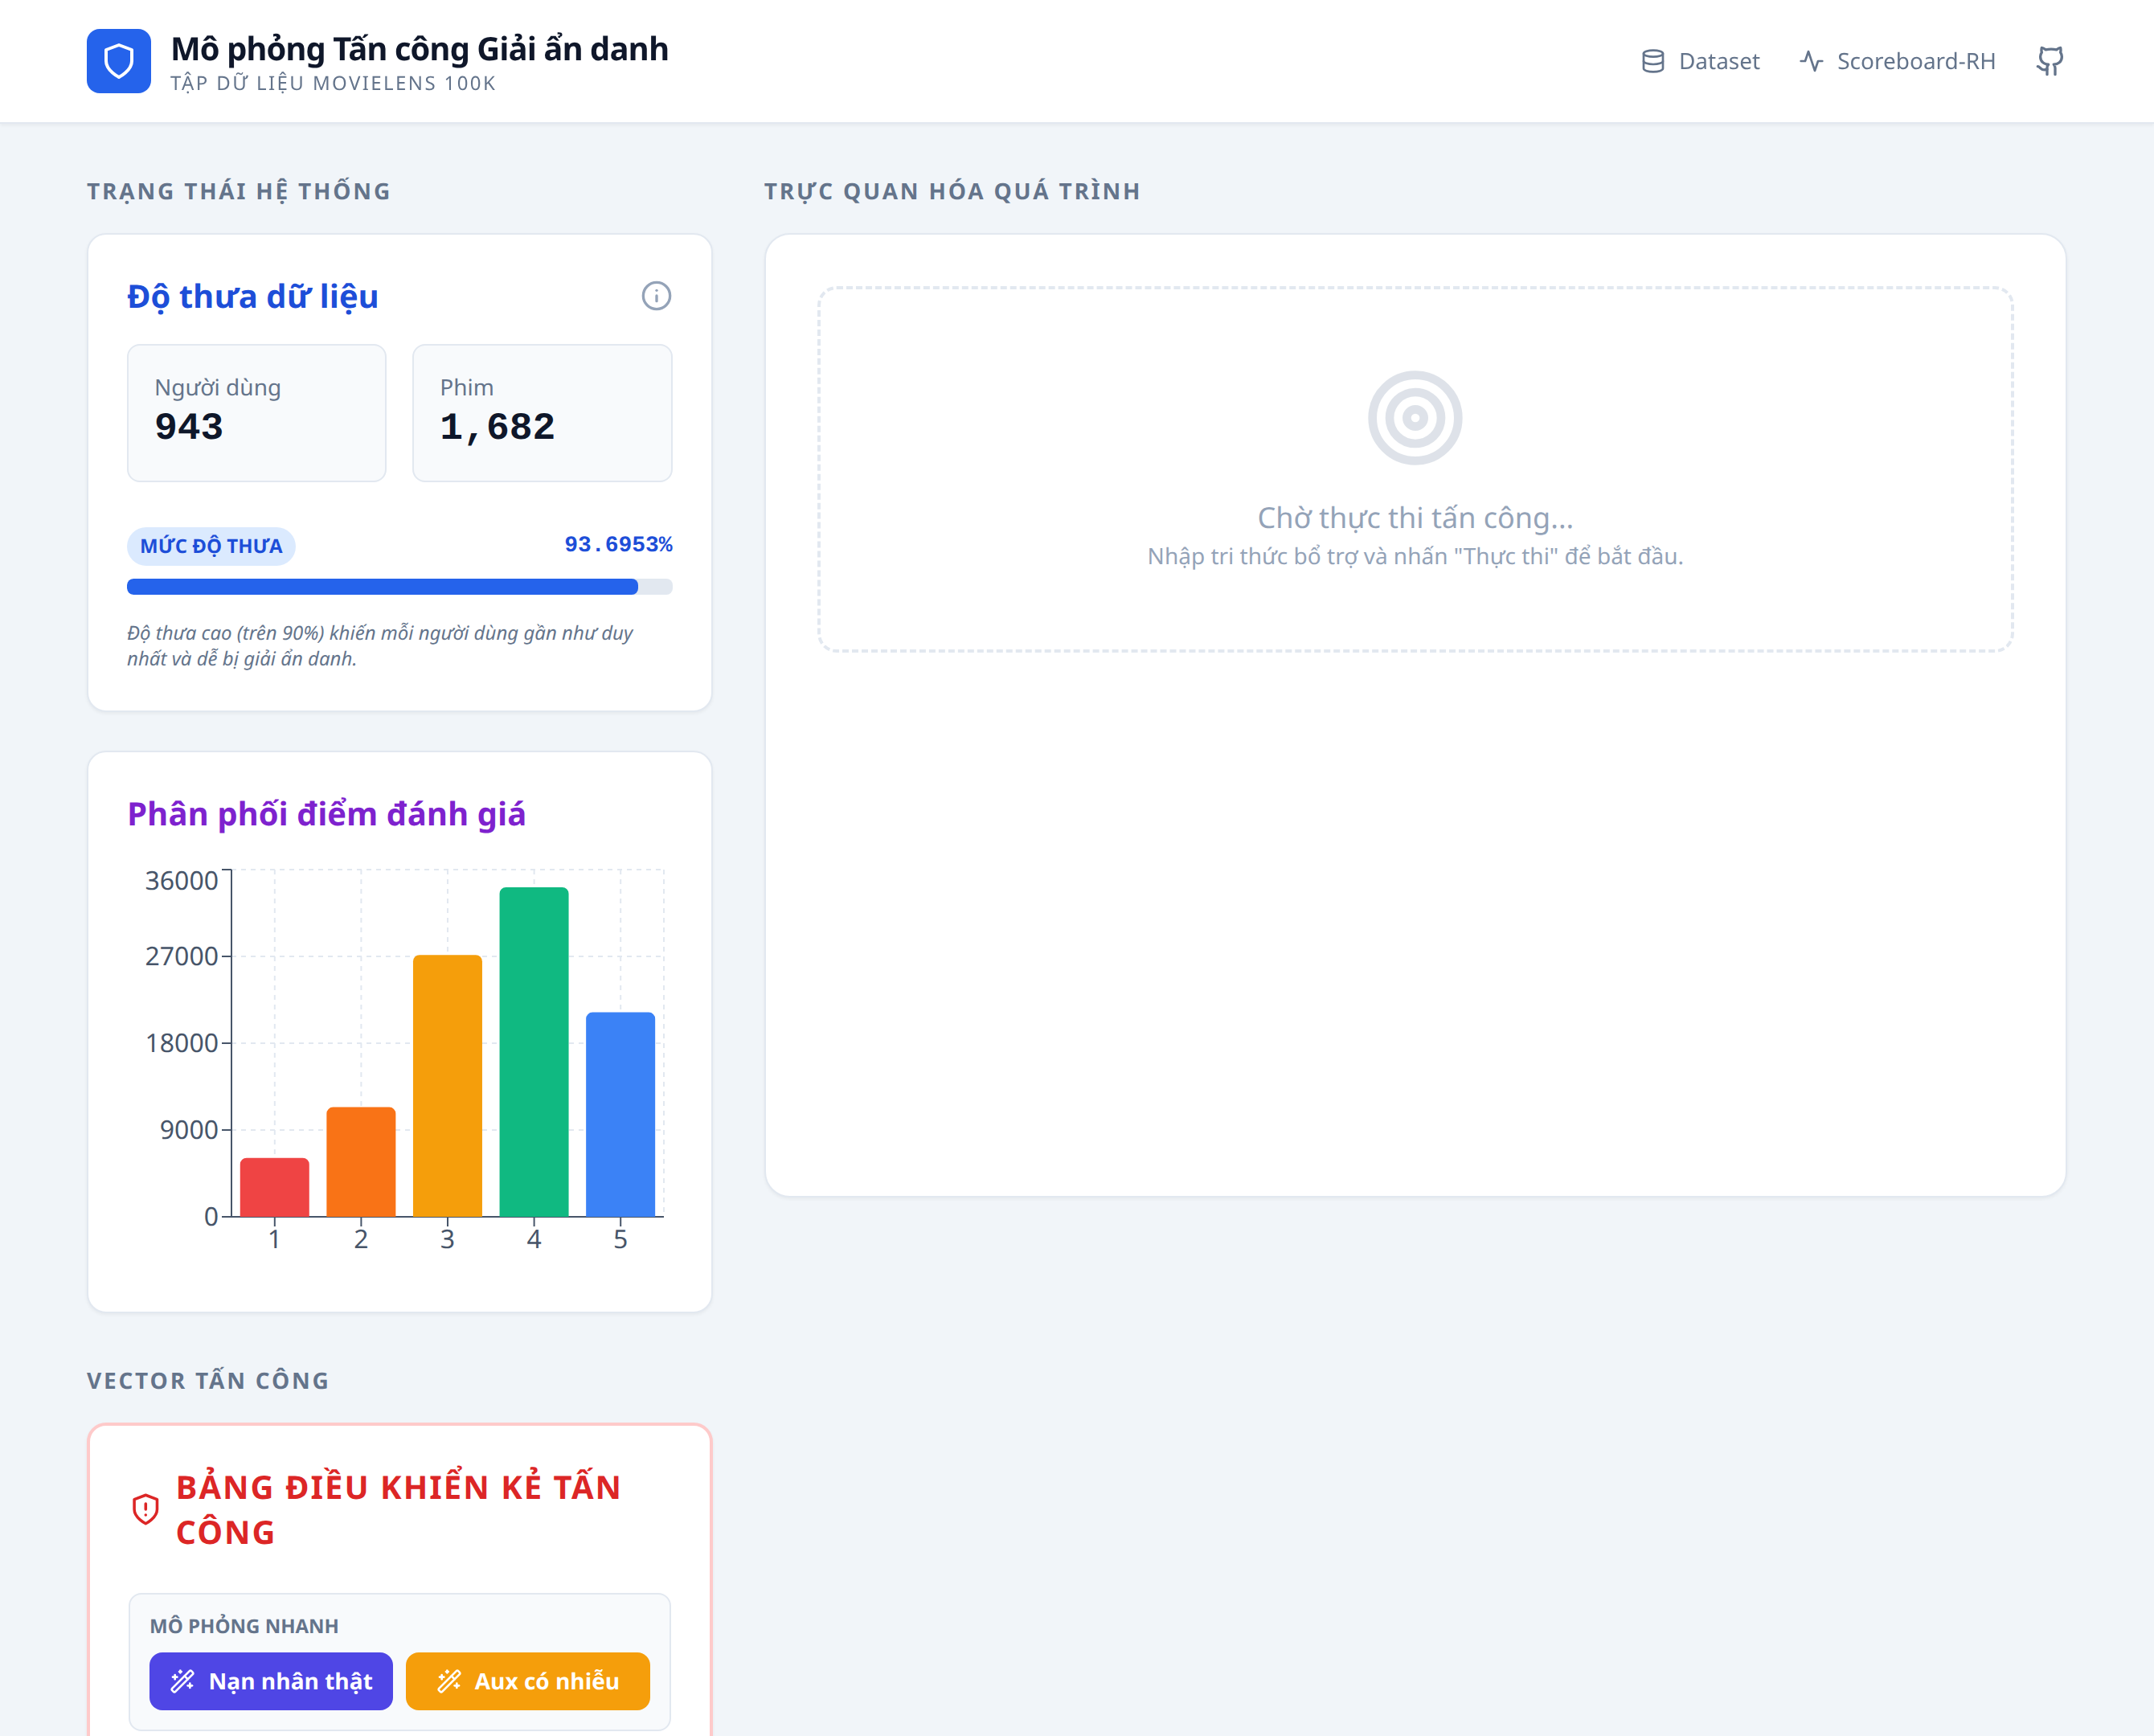
\includegraphics[width=0.95\linewidth]{figures/ui_01_overview.png}
\caption{Màn hình chính: thống kê độ thưa và bảng điều khiển kẻ tấn công}
\label{fig:ui_overview}
\end{figure}

\subsection{Nạp tri thức bổ trợ}
Chúng em dùng nút ``Nạn nhân thật'' để hệ thống lấy ngẫu nhiên dấu vân tay của một người dùng có thật. Hình~\ref{fig:ui_aux} cho thấy bốn phim được nạp vào bảng \textit{Thông tin đã biết}, mỗi phim kèm điểm, ngày, số người xem (support) và trọng số $wt(i)$. Có thể thấy các phim ít người xem (support nhỏ) được gán trọng số lớn hơn - đúng công thức~(\ref{eq:weight}).

\begin{figure}[!htb]
\centering
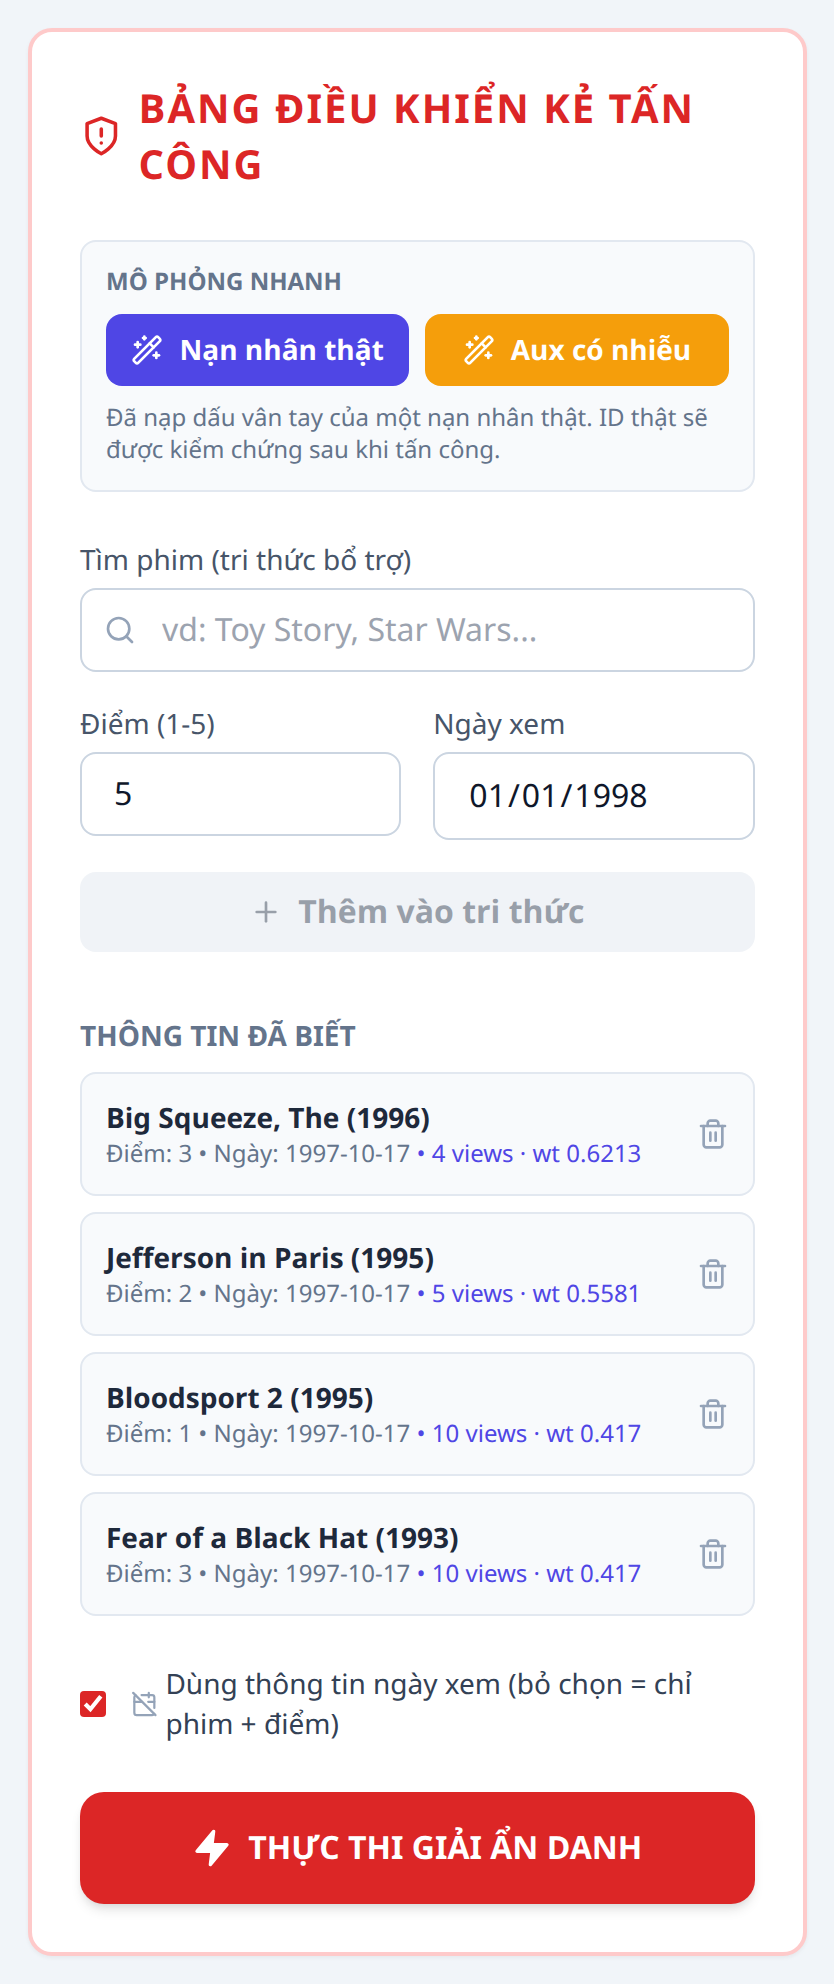
\includegraphics[width=0.46\linewidth]{figures/ui_02_aux_loaded.png}
\caption{Bảng điều khiển sau khi nạp aux: mỗi phim hiển thị support và trọng số độ hiếm}
\label{fig:ui_aux}
\end{figure}

\subsection{Kết quả định danh}
Sau khi nhấn ``Thực thi giải ẩn danh'', thuật toán xác định chính xác nạn nhân (Hình~\ref{fig:ui_result}): User \#373, eccentricity $3{,}8333$ (vượt xa ngưỡng $1{,}5$), độ tương tự $0{,}9886$. Đáng chú ý, không gian ứng viên chỉ còn 24 người - vì bốn phim hiếm trong aux đã thu hẹp đám đông xuống rất nhanh.

\begin{figure}[!htb]
\centering
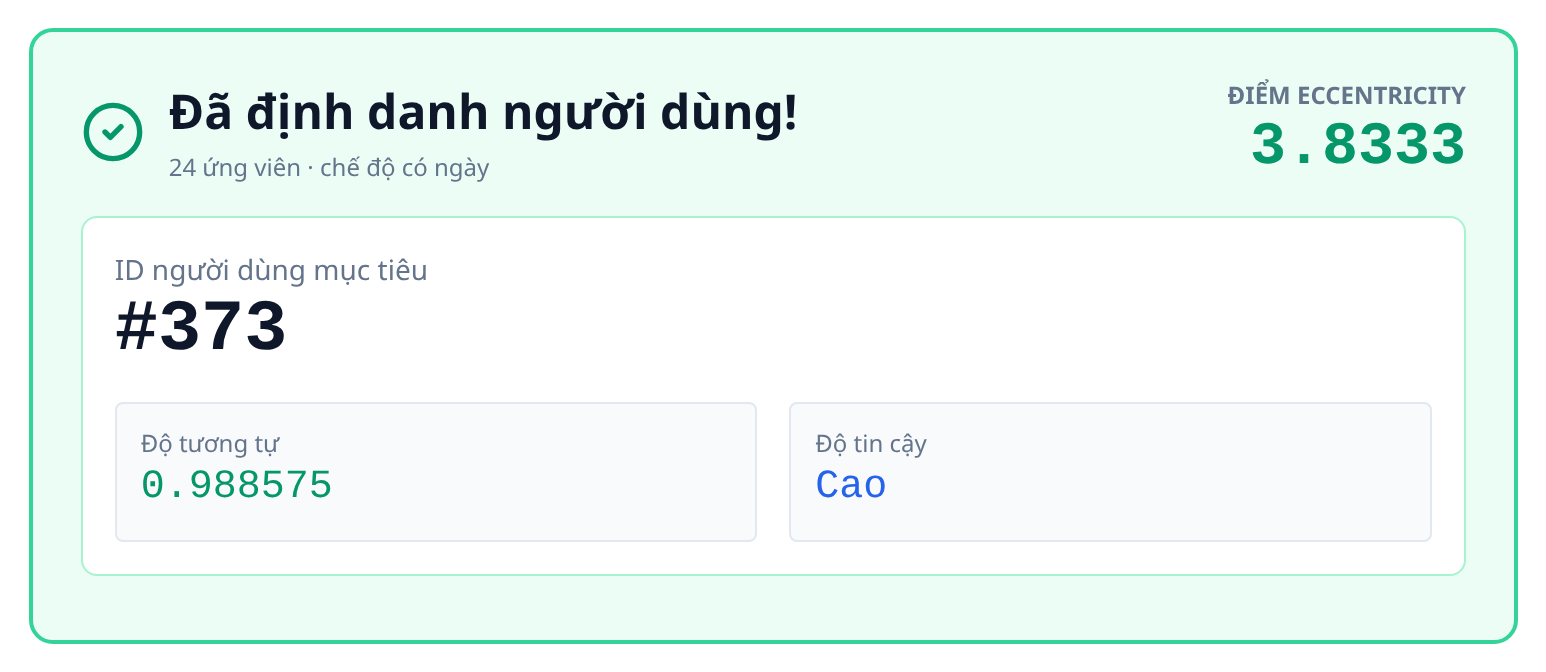
\includegraphics[width=0.95\linewidth]{figures/ui_03_result_identified.png}
\caption{Định danh thành công User \#373 với eccentricity $3{,}8333$}
\label{fig:ui_result}
\end{figure}

Quan trọng hơn, hệ thống phơi bày toàn bộ lịch sử xem phim của người này trong bảng \textit{Lịch sử riêng tư bị phơi bày} (Hình~\ref{fig:ui_history}) - 233 lượt đánh giá mà kẻ tấn công ban đầu hoàn toàn không biết. Đây chính là biểu hiện trực quan của ``rò rỉ riêng tư'': từ 4 mẩu thông tin, kẻ tấn công thu được toàn bộ chân dung hành vi của nạn nhân.

\begin{figure}[!htb]
\centering
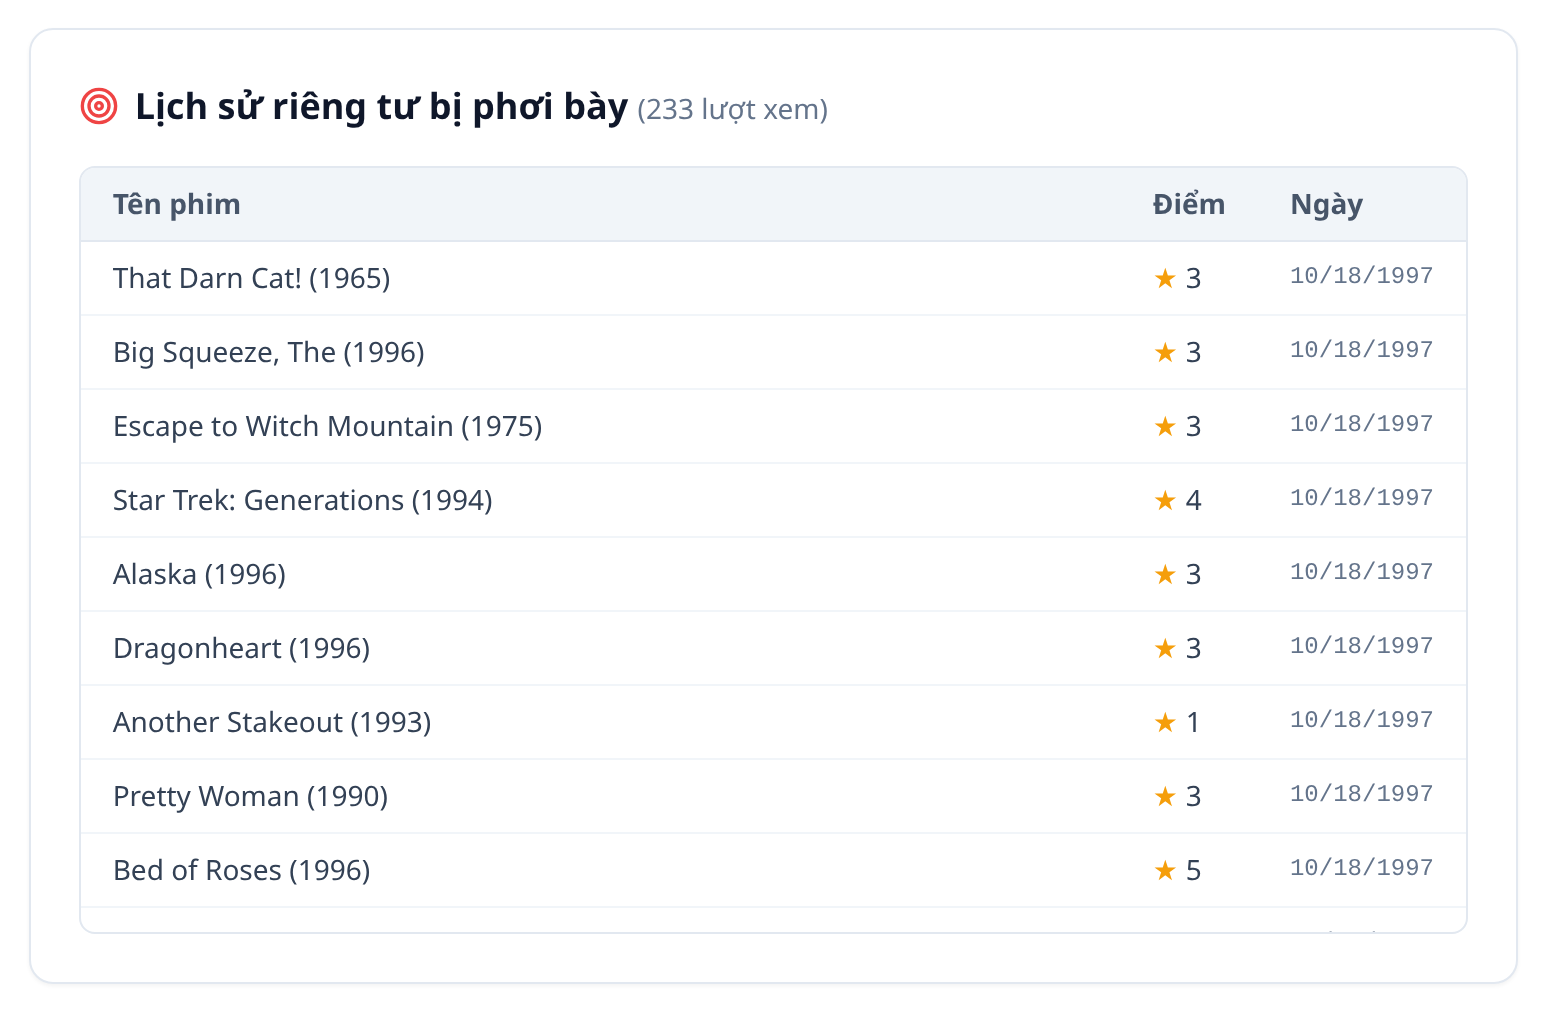
\includegraphics[width=0.82\linewidth]{figures/ui_04_exposed_history.png}
\caption{Lịch sử riêng tư của nạn nhân bị phơi bày hoàn toàn (233 lượt xem)}
\label{fig:ui_history}
\end{figure}

Hình~\ref{fig:ui_cand} là bảng xếp hạng \textit{Các ứng viên hàng đầu}: ứng viên hạng nhất (độ tương tự $\approx 0{,}99$) bỏ xa các ứng viên còn lại - minh họa trực quan ý nghĩa của eccentricity và lý do thuật toán tự tin kết luận.

\begin{figure}[!htb]
\centering
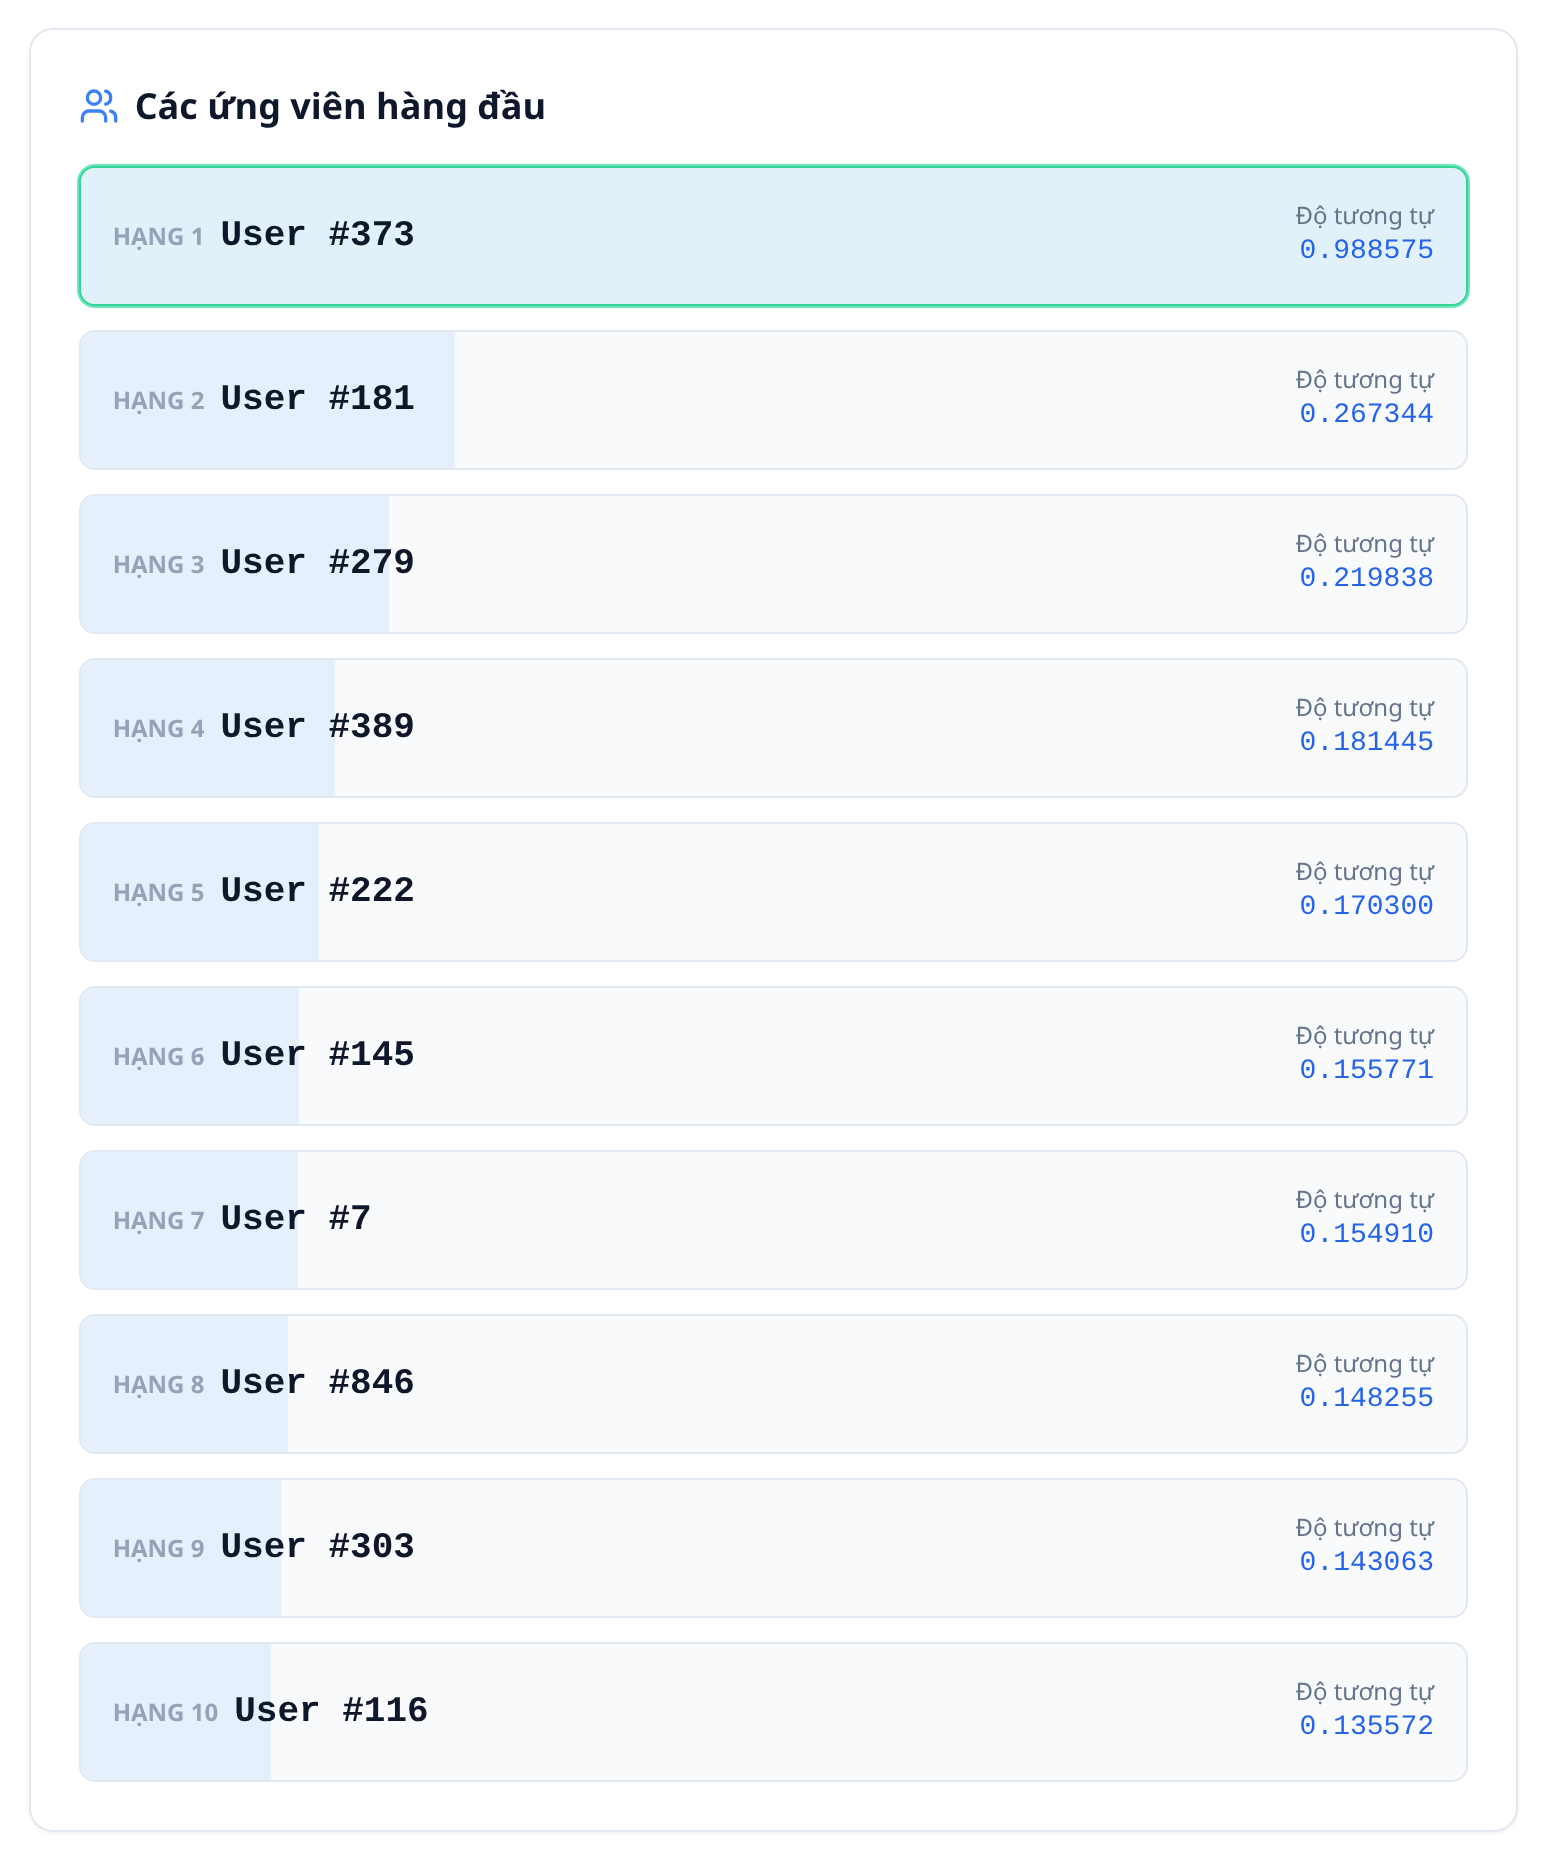
\includegraphics[width=0.80\linewidth]{figures/ui_06_top_candidates.png}
\caption{Bảng xếp hạng ứng viên: hạng nhất nổi bật hẳn so với phần còn lại}
\label{fig:ui_cand}
\end{figure}

\subsection{Tính bền vững trước thông tin nhiễu}
Để kiểm chứng tính bền vững, chúng em dùng nút ``Aux có nhiễu'': hệ thống lấy 6 phim của một nạn nhân thật nhưng cố ý làm sai điểm $\pm 1$ và sai ngày $\pm 14$ ngày. Dù vậy, thuật toán vẫn định danh đúng (Hình~\ref{fig:ui_noisy}): User \#278, eccentricity $5{,}1695$. Điều này xác nhận đặc tính ``robust'' cốt lõi: tấn công không đòi hỏi tri thức bổ trợ chính xác.

\begin{figure}[!htb]
\centering
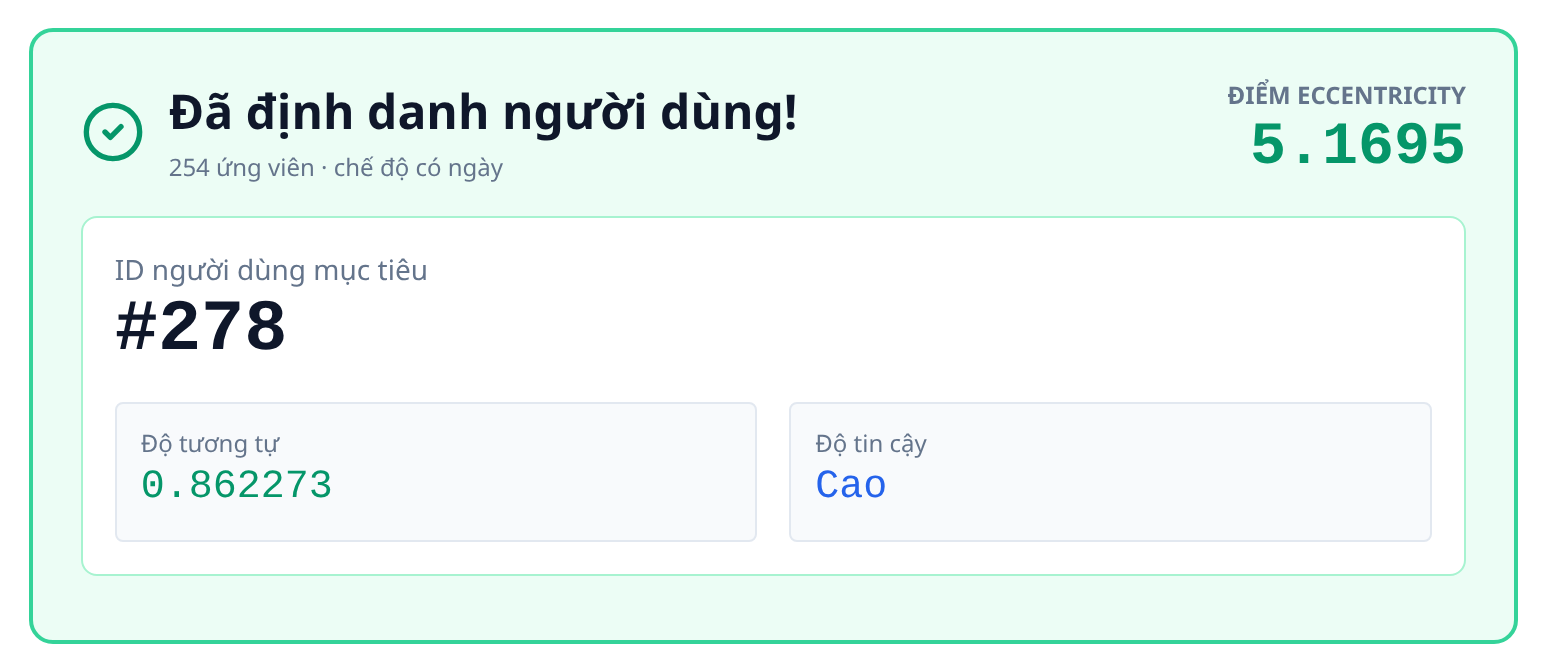
\includegraphics[width=0.95\linewidth]{figures/ui_05_robust_noisy.png}
\caption{Vẫn định danh đúng dù aux có nhiễu ($\pm 1$ điểm, $\pm 14$ ngày)}
\label{fig:ui_noisy}
\end{figure}

\section{Kiểm chứng trên dòng lệnh}

Để minh bạch, chúng em cũng chạy trực tiếp engine trên dòng lệnh. Hình~\ref{fig:term_demo} cho thấy một phiên tấn công vào nạn nhân thật \#200 với 6 phim chính xác: trong số 782 ứng viên, thuật toán chọn đúng người với độ tương tự tuyệt đối $1{,}0$, eccentricity $4{,}2504$, và phơi bày 216 lượt xem phim.

\begin{figure}[!htb]
\centering
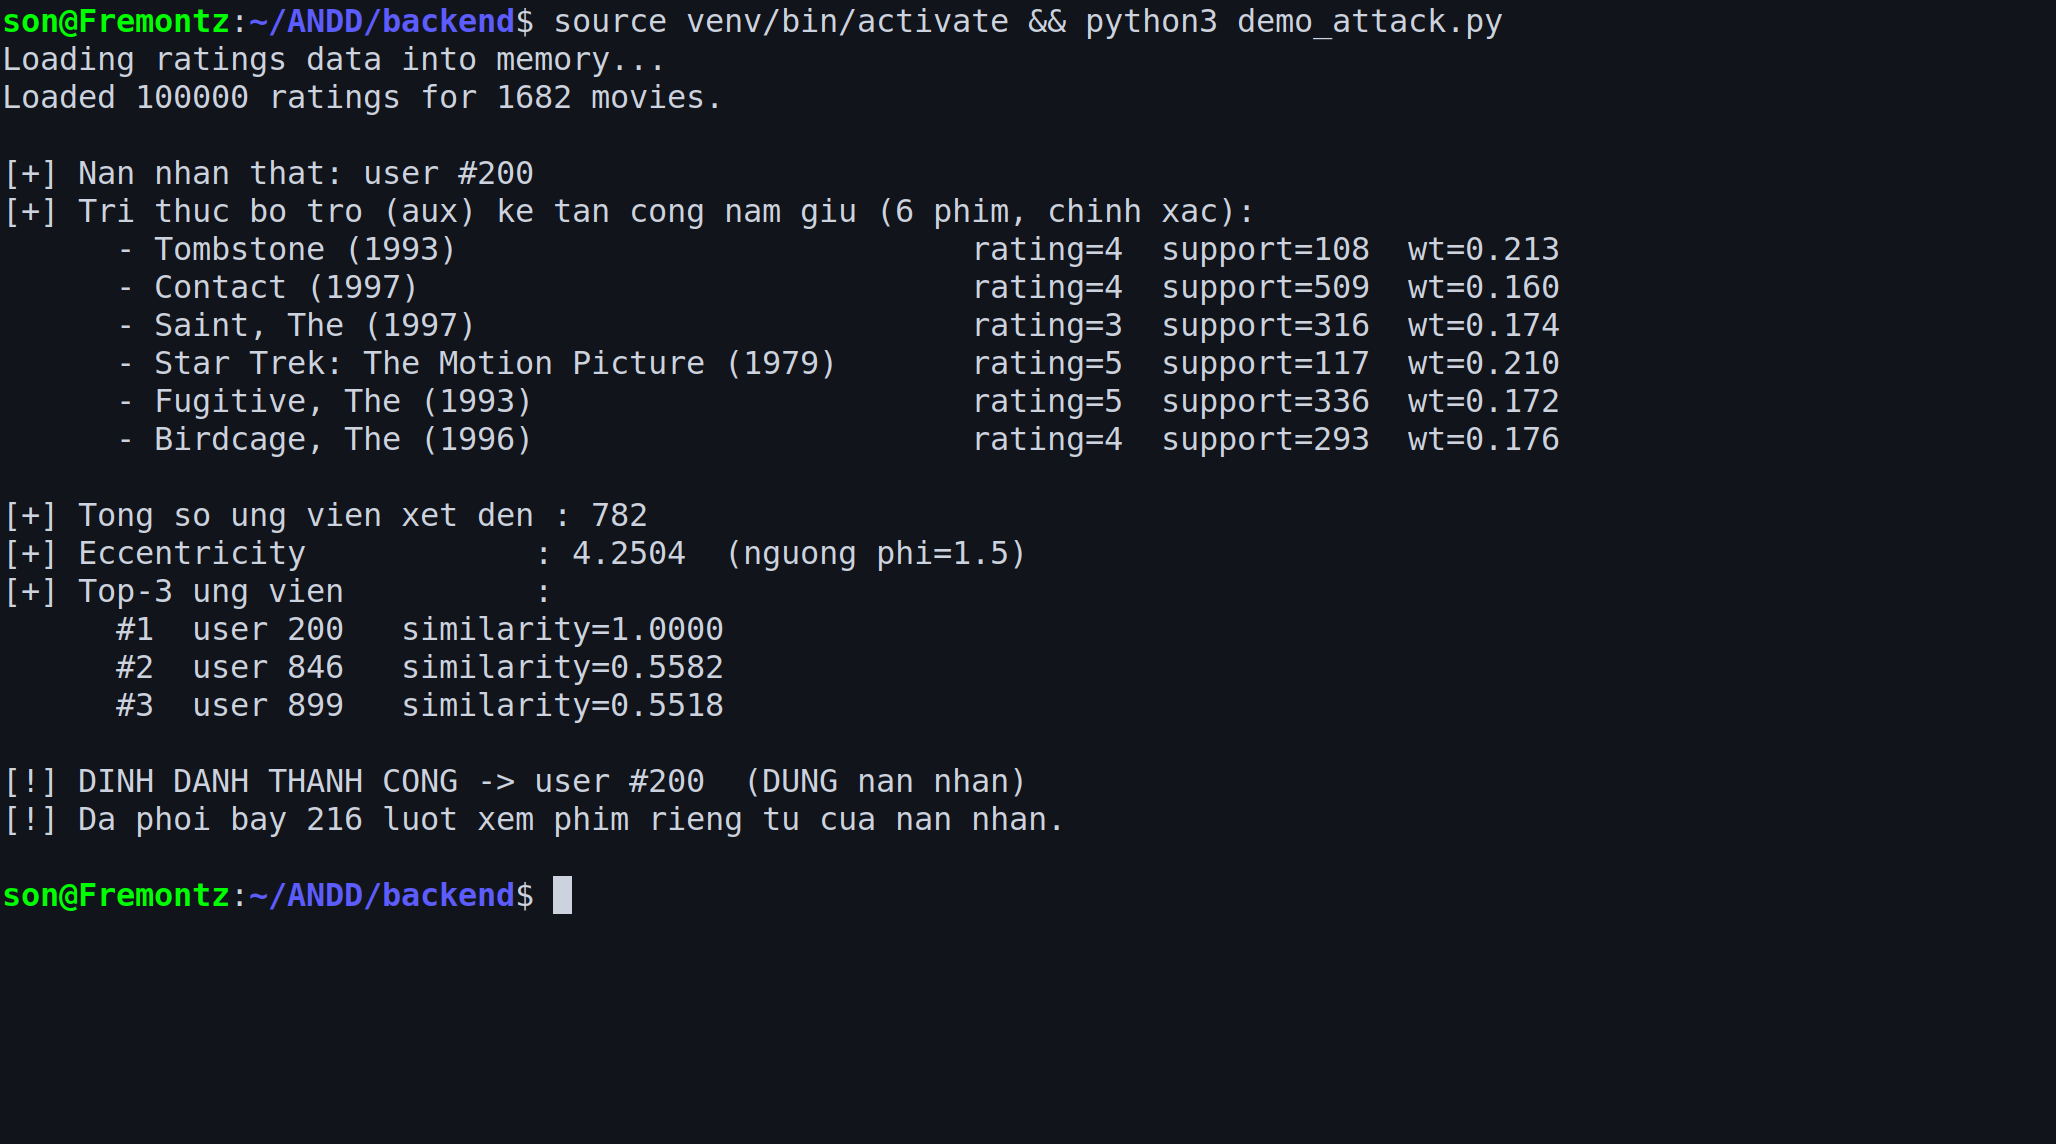
\includegraphics[width=0.92\linewidth]{figures/term_demo_attack.png}
\caption{Một phiên tấn công thật chạy trên dòng lệnh (nạn nhân \#200)}
\label{fig:term_demo}
\end{figure}

\section{Kết quả định lượng}

Phần này tái hiện kết quả chính của bài báo trên MovieLens. Chúng em chạy \texttt{experiment.py} trên 300 nạn nhân được chọn ngẫu nhiên (mỗi người đã xem $\ge 8$ phim), với năm mức số phim biết trước ($k \in \{2,3,4,6,8\}$) và bốn kịch bản. Kết quả thô in ở Hình~\ref{fig:term_exp} và tổng hợp ở Bảng~\ref{tab:results}.

\begin{figure}[!htb]
\centering
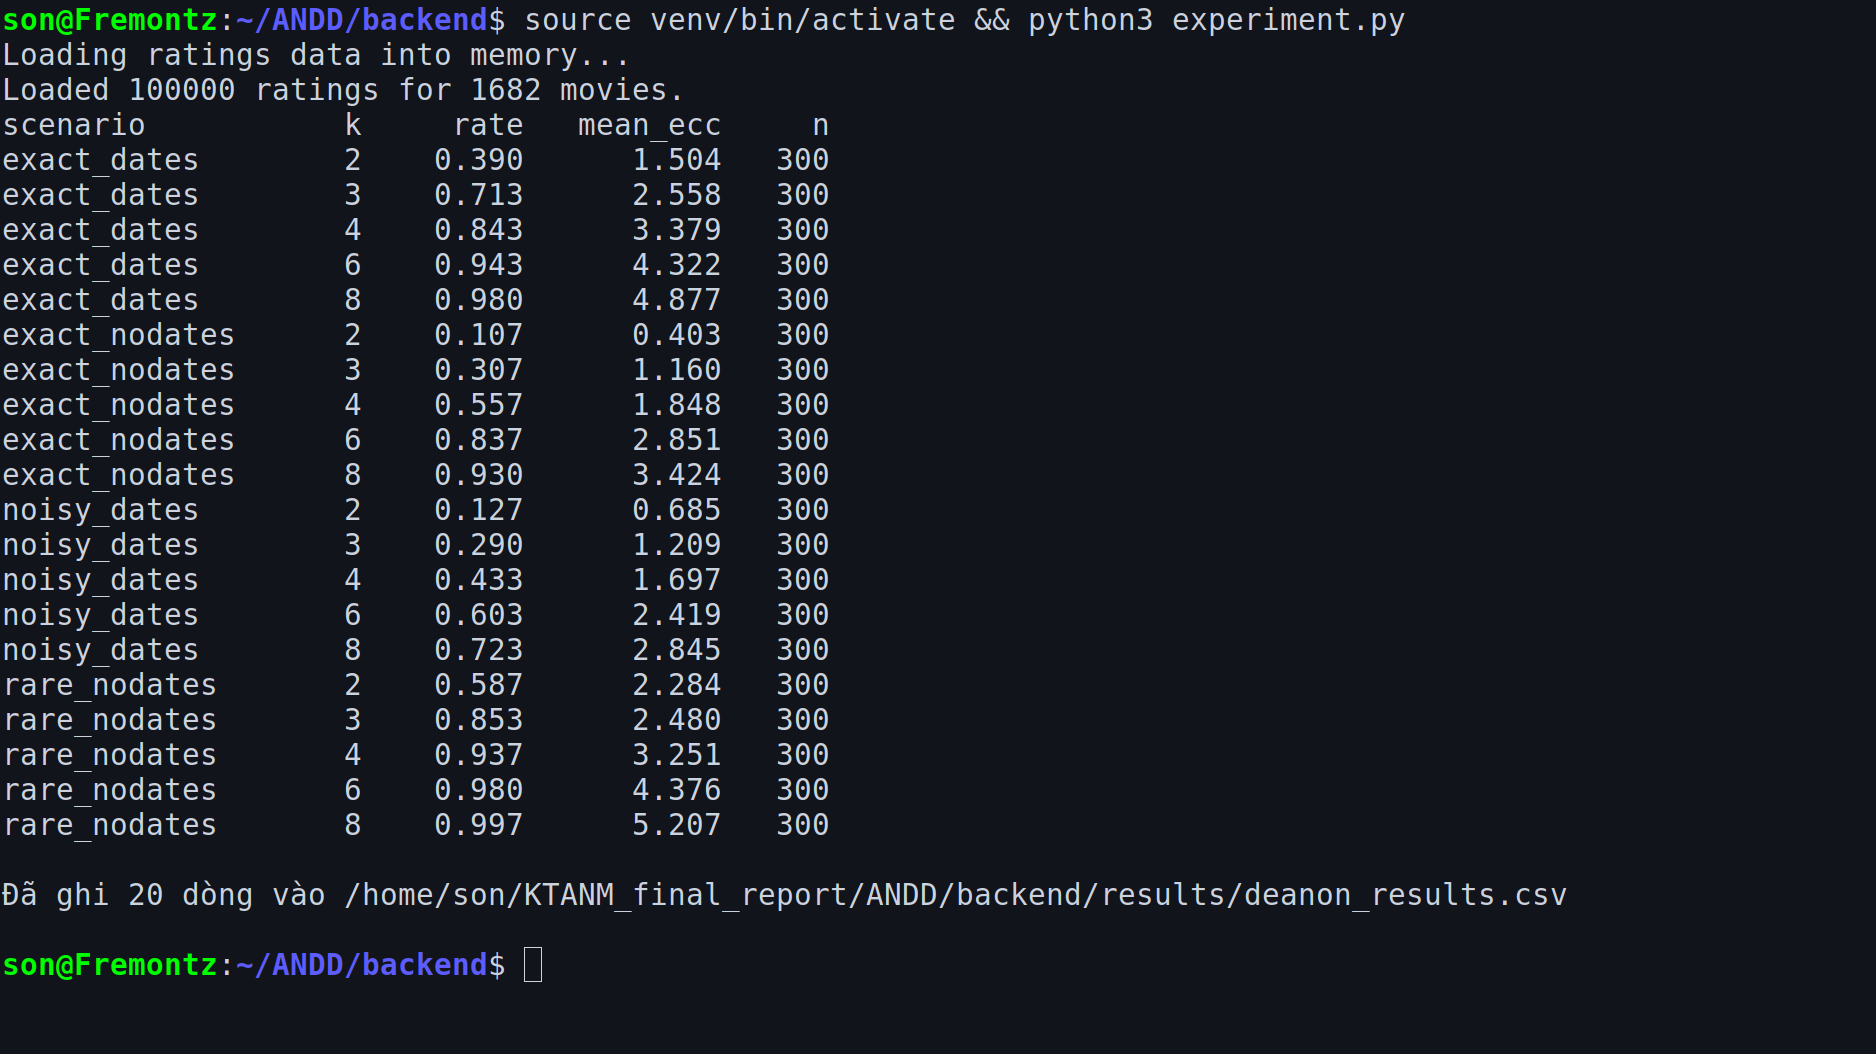
\includegraphics[width=0.82\linewidth]{figures/term_experiment.png}
\caption{Kết xuất (log) phiên chạy thực nghiệm trên 300 nạn nhân tại giao diện dòng lệnh, 4 kịch bản $\times$ 5 mức số phim}
\label{fig:term_exp}
\end{figure}

\begin{table}[!htb]
\centering
\caption{Tỉ lệ định danh đúng (\%) theo số phim biết trước và kịch bản}
\label{tab:results}
\renewcommand{\arraystretch}{1.3}
\begin{tabularx}{\linewidth}{X c c c c c}
\toprule
\textbf{Kịch bản} & \textbf{2 phim} & \textbf{3 phim} & \textbf{4 phim} & \textbf{6 phim} & \textbf{8 phim} \\
\midrule
Chính xác + có ngày        & 39{,}0 & 71{,}3 & 84{,}3 & 94{,}3 & \textbf{98{,}0} \\
Chính xác, không ngày      & 10{,}7 & 30{,}7 & 55{,}7 & 83{,}7 & 93{,}0 \\
Nhiễu ($\pm$1 điểm, $\pm$14 ngày) & 12{,}7 & 29{,}0 & 43{,}3 & 60{,}3 & 72{,}3 \\
Ưu tiên phim hiếm, không ngày & \textbf{58{,}7} & 85{,}3 & 93{,}7 & 98{,}0 & 99{,}7 \\
\bottomrule
\end{tabularx}
\end{table}

Hình~\ref{fig:chart_rate} và~\ref{fig:chart_ecc} trực quan hóa Bảng~\ref{tab:results} và eccentricity trung bình tương ứng.

\begin{figure}[!htb]
\centering
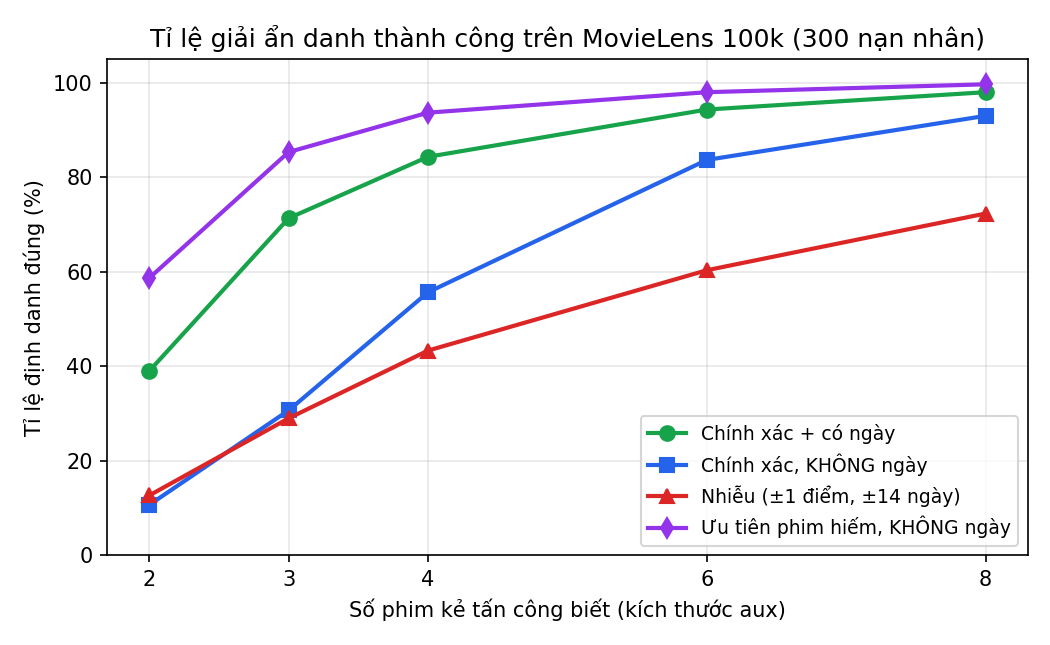
\includegraphics[width=0.85\linewidth]{figures/success_rate.png}
\caption{Tỉ lệ định danh thành công theo lượng tri thức bổ trợ}
\label{fig:chart_rate}
\end{figure}

\begin{figure}[!htb]
\centering
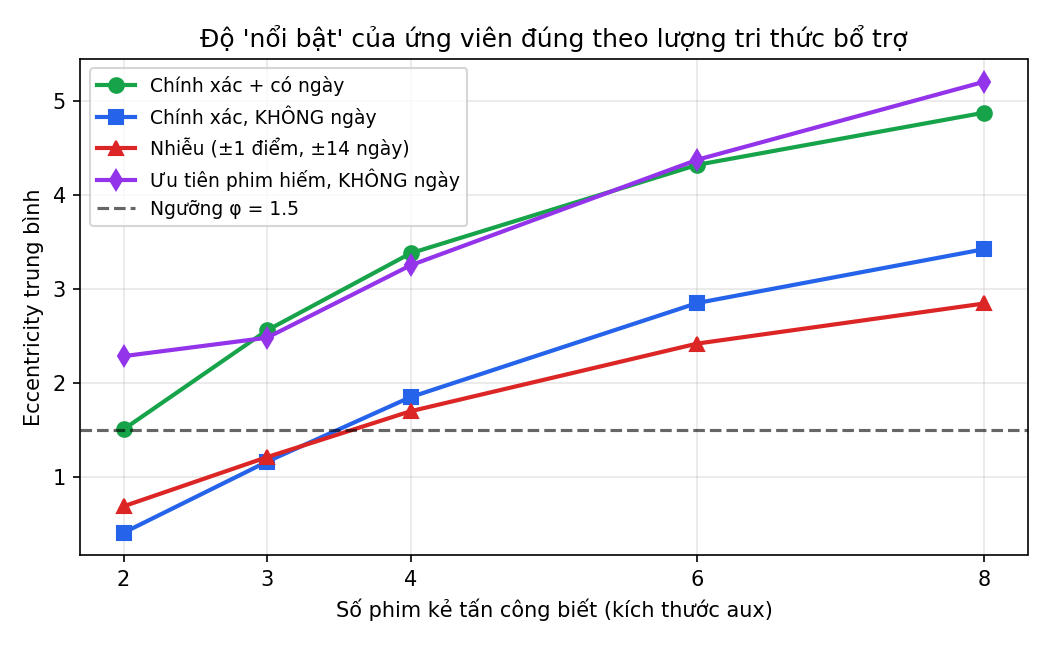
\includegraphics[width=0.85\linewidth]{figures/eccentricity.png}
\caption{Eccentricity trung bình theo lượng tri thức bổ trợ (đường nét đứt là ngưỡng $\phi=1{,}5$)}
\label{fig:chart_ecc}
\end{figure}

\section{Phân tích kết quả}

Các con số thật trên MovieLens tái hiện trung thực những kết luận của bài báo gốc:

\renewcommand{\labelitemi}{$-$}
\begin{itemize}
	\item \textbf{Càng nhiều tri thức, càng dễ định danh.} Với 8 phim chính xác kèm ngày, tỉ lệ định danh đúng đạt 98\% - rất gần con số 99\% mà bài báo công bố trên Netflix.
	\item \textbf{Ngày xem là thông tin giá trị nhưng không bắt buộc.} Bỏ thông tin ngày làm tỉ lệ giảm (ví dụ với 4 phim: từ $84{,}3\%$ xuống $55{,}7\%$), nhưng khi biết đủ 8 phim vẫn đạt $93\%$. Quyền riêng tư không được cứu vãn chỉ bằng cách giấu ngày.
	\item \textbf{Tấn công bền vững trước nhiễu.} Ngay cả khi điểm sai $\pm 1$ và ngày sai $\pm 14$ ngày, 8 phim vẫn cho $72{,}3\%$. Tri thức bổ trợ \textit{không cần chính xác}.
	\item \textbf{Phim hiếm là vũ khí mạnh nhất.} Khi ưu tiên phim ít người xem, chỉ 2 phim đã đủ định danh $58{,}7\%$ - cao hơn cả việc biết 4 phim phổ biến. Điều này khẳng định vai trò của trọng số độ hiếm $wt(i)$: một bộ phim nghệ thuật ít người biết tiết lộ nhiều hơn nhiều so với một bom tấn.
	\item \textbf{Eccentricity tăng đều theo lượng tri thức} (Hình~\ref{fig:chart_ecc}), cho thấy ứng viên đúng ngày càng ``nổi bật'' và cơ chế tự kiểm soát sai số hoạt động ổn định.
\end{itemize}

\section{Tình huống thất bại và ý nghĩa của ngưỡng}

Không phải mọi cuộc tấn công đều thành công - và đó là chủ ý thiết kế. Khi tri thức bổ trợ ít hoặc chỉ gồm phim phổ biến, nhiều người dùng có hồ sơ tương tự nhau, eccentricity tụt xuống dưới $1{,}5$ và thuật toán từ chối định danh thay vì đoán bừa. Trong một thực nghiệm với 5 phim phổ biến kèm nhiễu, ứng viên hạng nhất tuy đúng là nạn nhân nhưng eccentricity chỉ đạt $1{,}4995$ - sát ngưỡng - nên hệ thống vẫn báo ``không đủ tin cậy''. Cơ chế ngưỡng này giữ tỉ lệ dương tính giả ở mức thấp, khiến mỗi lần ``định danh thành công'' đều có độ tin cậy cao - đây chính là điều làm cho tấn công trở nên \textit{nguy hiểm} trên thực tế.
